\documentclass[sigconf]{acmart}
\usepackage{booktabs} % For formal tables
\usepackage{graphicx}
\usepackage{CJKutf8}
\usepackage{multirow}

\begin{document}
\title{Persuasively Explainable Recommendation}

\author{Lingting Lin}
\affiliation{%
  \institution{Department of Computer Science, Xiamen University}
  \city{Xiamen}
  \state{China}
}
\email{linlingting@stu.xmu.edu.cn}

\author{Chen Lin}
\affiliation{%
  \institution{Department of Computer Science, Xiamen University}
  \city{Xiamen}
  \state{China}
}
\email{chenlin@xmu.edu.cn}


\begin{abstract}
In the e-commerce environment, it is a personalized service to recommend suitable products according to the shopping scene of the user. We hope to provide users with an explainable and persuasive recommendation reason when recommending products, that is, why they should recommend this product, and motivate online purchasers to make successful purchases through persuasive descriptions. In this contribution we present our system by combinning weak supervision frame with generate model.  We first select the persuasive sentences from corpus as the training data of our generate model through weak supervision. Then through our proposed model yield persuasive sentence. We conduct comprehensive experiments on real sets. Compared with state-of-the-art methods, our framework produces sentences with higher ROUGE and BLEU scores and more attractive and persuasive.

\end{abstract}

\keywords{persuasive, explainable,recommendation}


\maketitle

\section{INTRODUCTION}
%1.可解释推荐在电商很重要
%2.persuasive在可解释推荐中很重要,举例子:容易买单
%3.现有工作对可解释推荐的persuasive很少,呈现形式有图片,概念等,没人考虑用句子解释
%4.与最新工作的差别
%5.我们的目标,为什么能做,根据用户当前行为+淘宝场景图谱,生成推荐,我们是第一篇这么做的
%6.挑战

With the rapid development of e-commerce, more and more customers choose to purchase goods on the Internet. In mass goods, how to attract customers' attention through product description and strive for customers' stay time is a means to stand out from a large number of merchants. At present, the generation of product descriptions mainly relies on manual generation, and there is a problem that the amount of products covered is small and the cost is high. In recent years, deep learning has made breakthroughs in many fields such as image, natural language processing, and information retrieval. If we can generate persuasive product descriptions through deep learning, we can save costs and also improve the quality of content. Because a person's knowledge is limited, the generated vocabulary is limited. By learning a large amount of data, the machine-generated content can far exceed one's information.

%challenge
Two challenges arise in generating persuasive and explainable recommendations for recommended products automatically .

The first challenge lies in getting training data. It is almost impossible to get a tag corpus, the data is a description of the product, and the tag is whether these descriptions are persuasive. Only the corpus contains descriptions of the products, but there is no guarantee that these sentences are persuasive. We need to choose persuasive sentences from these corpus as our training set.

The second challenge is related to the description of the scene. In our corpus, there are many sentences with only product descriptions, no descriptions of related scenes, but with the description of the scene is the sentence we really want. We need to design new module for this purpose.

%idea
Our goal is to generate persuasive recommendation reason containing scene descriptions when recommending products. To solve the first challenge, we use a weak supervision framework to select persuasive sentences. Weak supervision frameword mark the data without the user to manually mark any training data. In this way, we do not cost time to label mass of data manually.

To solve the second challenge, we propose a global local module: a specific module that focuses on the description of the scene. It has two parts, the global part is to learn the text description of all products on all texts, and the local part is to learn the scene-specific description through the local module. Through the weighted sum of these two parts, the generated sentence also has a description of the scene while describing the product.

%contributions
Our contributions are three folds. (1) We take the problem of generating persuasive descriptions as sequence to sequence model . The source text are scene and attribute about the product, the target text are persuasive description within scene about the product. (2) we use a weak supervision framework to select persuasive sentences as the training set of the model, which avoids a lot of manual labeling work. (3) Our system introduces a global-local module, so that the automatically generated description sentences for products can be described with scenes. 

%paper structure
This paper is organized as follows. We briefly survey the related work in Sec.~\ref{sec:related}. In Sec.~\ref{sec:architecture}, we first introduce the architecture of our system and describe the weak supervision and our global-local-copy model. We present and analyze the experimental results on a real data set in Sec.~\ref{sec:experiment}. We conclude our work and suggest future directions in Sec.~\ref{sec:conclusion}.

\section{RELATED WORK}\label{sec:related}
%1.explainable recommendation
%2.persuasive argue

In recent years, there have been many studies on natural language processing, including poetry creation \cite{Colton2012Full,Oliveira2015Tra,Ghazvininejad2016Generating,Yi2017Generating,Zhang2014Chinese,wang2016chinese},machine translation \cite{Kalchbrenner2016Neural,Zhou2016Deep,Wu2016Google}, and so on. A persuasive and explainable recommendation reason for the generation of goods, similar to the above two questions, is a sequence model. In fact, most ML research usually focuses on predictive tasks, but rarely provides explanations for them. However, many customers need to rely on the recommendation reasons provided by the system to be firm in their determination to purchase the item.

The traditional explainable recommendation method has content-based recommendation and collaborative filtering. \cite{vig2009tagsplanations,sigurbjornsson2008flickr} used tags as content features for recommendations and generate corresponding explanations. Collaborative filtering is divided into user-based collaborative filtering and item-based collaborative filtering. \cite{herlocker2000explaining, gedikli2014should,sarwar2001item} provided an explanation using the ratings of its neighbors or its similar items. In recent years, many models have attempted to use textual information to generate textual explanations for recommendations. One is to extract commodity features as an explanation, such as \cite{wu2015flame} used topic models to explain recommendations, \cite{zhang2017entity} found the related entities and gave conceptual explanation, the other is to generate complete sentences as an explanation, such as \cite{ozbal2013brainsup} generated textual explanation based on fixed templates, \cite{munigala2018persuaide} based on linguistic creativity to generate various forms of sentences. 

\section{SYSTEM ARCHITECTURE}\label{sec:architecture}
We take the corpus of product as the input of our system, and produces a persuasive sentence with the scene description of the product. Fig.~\ref{fig:system-architecture} shows an overview of the proposed system architecture with two major steps: (1) Given the corpus of product,the first step is to select the persuasive sentences as the training data of our model, (2) identify the scene name, product name, cpv data \footnote{Cpv is a collection of values of the attributes of the product. Here, only the value of the product attributes is in the sentence it can be extracted.} from the selected sentence as the input of our model,then yield persuasive sentence. In this section, we first introduce the weak supervision method for selecting the persuasive sentences. We then present our global-local-copy model in detail.  

\begin{figure}
    \centering
    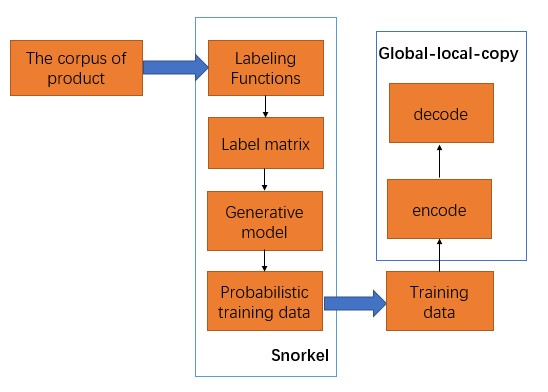
\includegraphics[width=8cm,height=5cm]{system-architecture.jpg}
\caption{System Architecture}\label{fig:system-architecture}
\end{figure}

\subsection{Resources Used}
% Data set
We use the list of product recommendation reasons as our dataset. The corpus are generated by high quality person.But the quality of the original dataset is far from ideal, there are many recommended reasons are even the original title of the product, so we need to filter the training data.

\subsection{Weak Supervision}
% Weak Supervision
Manual labeling is very time consuming, so we use the Snorkel \cite{ratner2017snorkel} weak supervision method to mark the data without the user to manually mark any training data. Rather than hand-labeling training data, users of Snorkel write labeling functions(LF), which allow them to express various weak supervision sources such as patterns, heuristics, external knowledge bases, and more. We wrote ten labeling functions based on the characteristics of persuasive sentences, is shown in Tab.~\ref{table:LF}. Among them, the labels of the first five functions are positive and the rest are negative.

\begin{table}
  \caption{Labeling Functions}
  \label{table:LF}
  \begin{tabular}{p{2.5cm}p{5cm}}
    \toprule
    Labeling Functions & Description\\
    \midrule
    %正类
    is\_neat & Sentence is neat\\
    has\_modal & Sentence has modal particle\\
    four\_word & Sentence contains a four-word structure \\
    dot\_word & The comma is followed by
        \begin{CJK*}{UTF8}{gbsn}
            "让/使/为/给"
        \end{CJK*}
        or verbs\\
    end\_exclamation & Sentence ends with an exclamation point\\
    %负类
    no\_adj\_and\_adv & Sentence has no adjectives and adverbs\\
    other\_words & Sentence contains characters other than Chinese, English, numbers, and specified symbols
        \begin{CJK*}{UTF8}{gbsn}
            (。,?!、;:).
        \end{CJK*}\\
    tree\_depths & the depth of the dependency tree is greater than 10\\
    clause\_num & the number of clauses is greater than 10\\
    token\_num & the number of word segments is greater than 10\\
  \bottomrule
\end{tabular}
\end{table}

Next, Snorkel automatically learns a generative model over the labeling functions,the output of Snorkel is a set of probabilistic labels. The statistics about the resulting label matrix is shown in Tab.~\ref{table:LabelMatrix}. \textbf{Coverage} is the fraction of candidates that the labeling function emits a non-zero label for. \textbf{Overlap} is the fraction candidates that the labeling function emits a non-zero label for and that another labeling function emits a non-zero label for. \textbf{Conflict} is the fraction candidates that the labeling function emits a non-zero label for and that another labeling function emits a conflicting non-zero label for. We choose sentences with probabilistic labels are bigger than 0.5 and the words are less than 50 as the training set of our model.

\begin{table}
  \caption{Statistics about the resulting label matrix}
  \label{table:LabelMatrix}
  \begin{tabular}{p{2cm}p{1.5cm}p{1.5cm}p{1.5cm}}
    \toprule
    LFs & Coverage & Overlaps & Conflicts\\
    \midrule
    %正类
    is\_neat & 0.075185 & 0.060664 & 0.040715\\
    has\_modal & 0.022520 & 0.019763 & 0.004743\\
    four\_word & 0.418368 & 0.333411 & 0.061301 \\
    dot\_word & 0.607374 & 0.411911 & 0.118444\\
    end\_exclamation & 0.070130 & 0.061328 & 0.010403\\
    %负类
    no\_adj\_and\_adv & 0.113256 & 0.086246 & 0.063460\\
    other\_words & 0.060238 & 0.052460 & 0.049377\\
    tree\_depths & 0.004969 & 0.004637 & 0.004564\\
    clause\_num & 0.022300 & 0.022194 & 0.022154\\
    token\_num & 0.103537 & 0.077849 & 0.056611\\
  \bottomrule
\end{tabular}
\end{table}

\subsection{Background: Transformer}
Transformer~\cite{vaswani2017attention} is a network architecture based solely on an attention mechanism, dispensing with recurrence and convolutions entirely. Transformer have an encoder-decoder structure and both the encoder and decoder are composed of a stack of $N = 6$ identical layers.

\textbf{Encoder:} Each layer has two sub-layers. The first is a multi-head self-attention mechanism, and the second is a fully connected feed-forward network.

\textbf{Decoder:} In addition to the two sub-layers in each encoder layer, the decoder inserts a third sub-layer, which performs multi-head attention over the output of the encoder stack. 


\subsection{Global-Local-Copy Model}
Global-Local-Copy model is comprised of three modules which is based on Transformer architecture. Fig.~\ref{fig:model} illustrates the detailed model structure. Global-Local-Copy model is also with encoder-decoder structure. The encoder consists of global module and local module and the copy module is in decoder part. 

Our goal is to generate persuasive sentences with scene descriptions based on the scenes, products, and attributes given by the user. In our training set, some sentences have only product descriptions, no descriptions of related scenes, and some sentences are product descriptions in different scenarios. We use a global module to learn text descriptions of all products on all texts and learn scene-specific description through local modules. We want the output sentence to contain user-supplied input, so we also add the copy module to our model.

\textbf{Encoder:} We produce a global encoding $H^{global}$ of $X$ using a global encode part of Transformer and the local encoding is $H^{local}$. The outputs of the two modules are combined through a mixture layer to yield a global-local encoding $H$ of $X$. The left of Fig.~\ref{fig:model} illustrates the global-local modules encoder. 
\begin{figure*}
    \centering
    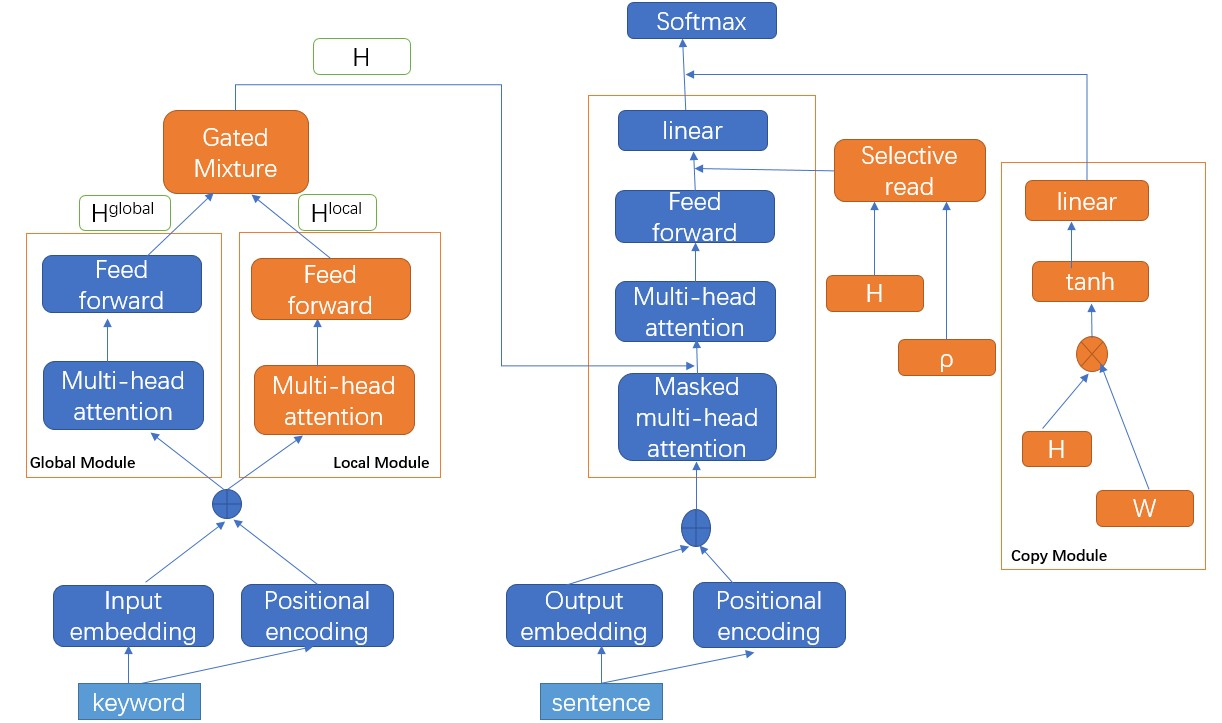
\includegraphics[width=12cm,height=8cm]{model2.jpg}
\caption{Global-Local-Copy Model}\label{fig:model}
\end{figure*}

\begin{equation}\label{equ:mixture}
    \mathbf{H} = \beta^s\mathbf{H}^{local} + (1-\beta^s)\mathbf{H}^{global}.
\end{equation}
Here, the scalar $\beta$ is a learned parameter between 0 and 1 that is specific to the scenario $s$.

\textbf{Decoder:} The copy module is in decoder module, the probability of generating any target word $y_t$, is given by the mixture of probabilities as follows

\begin{equation}\label{equ:mixture-prob}
    p(y_t) = p(y_t,g) + p(y_t,c)
\end{equation}

where $g$ stands for the generate-mode, and $c$ the
copy mode. the right of Fig.~\ref{fig:model} illustrates the copy module decoder. $H$ is global-local encoding the above-mentioned, $\zeta(y)$ is the weighted sum of hidden states $H$ corresponding to $y$, referred to as selective read in the right of Fig.~\ref{fig:model}. 

\begin{equation}\label{equ:zeta}
    \zeta(y) = \sum^{T}_{\tau = 1} \rho_\tau \textbf{h}_\tau 
\end{equation}

\begin{equation}\label{equ:rho}
    \rho_\tau = \left\{
        \begin{aligned}
        \frac{1}{K} p(x_\tau,\textbf{c}|\textbf{H}), \quad & x_\tau = y_t & \\
        0, \quad & otherwise &
        \end{aligned} 
        \right.
\end{equation}

where $K$ is equal to the number of positions with source keywords in the target sentence, $\tau$ is the index of source keywords, $T$ is the number of keywords, $t$ is the index of word in target sentence, and $p(x_\tau,\textbf{c}|\textbf{H})$ is the probability of the source keyword be copied in target sentence. 

The score of each mode is calculated:

\textbf{Generate-Mode}: first connect the output of the feed forward part of the transformer method and selective-read, and then $p(y_t,g)$ is calculated through the full connection. 

\textbf{Copy-Mode}: first calculate $\sigma(\textbf{H}\textbf{W})$, $\sigma$ is a non-linear activation function, here using the $tanh$ function. Next $p(y_t,c)$ is calculated through the full connection. 

\section{EXPERIMENTAL SETUP}\label{sec:experiment}
\subsection{Dataset}
In this paper,we focus on two sub-scenarios under the home: creative home and simple home. We select the description of the products in these two scenarios from the list of product recommendation reasons. We collected 150,743 sentences related to these products, after weak supervision, left 103,612 sentences. We chose sentences which keyword input only appears once as the test set. Training data format is shown in Tab.~\ref{table:format}. 

\begin{table}
\caption{Training data format }\label{table:format}
\begin{center}
\begin{tabular}{p{2.5cm}p{5cm}}
    \toprule
    Input & Output \\
    \midrule
    \begin{CJK*}{UTF8}{gbsn}
        创意,纸巾盒,欧式
    \end{CJK*} &
    \begin{CJK*}{UTF8}{gbsn}
        一款欧式风范榉木纸巾盒,盒身采用创意撞色设计,不仅能放杂物,还能作为桌面摆设,大中小三种尺寸可选,适合多种场合使用。
    \end{CJK*} \\
    \bottomrule
\end{tabular}
\end{center}
\end{table}

\subsection{Comparative Method}
%WWW这篇有一步寻找名词短语,我的替换方法是 形容词(1个或多个)+ 的 + 名词(0个或1个) 例如: 浪漫的荷花  这样子的词语
%None Phrase Selection部分,改成寻找【形容词(1个或多个)+ ‘的’ + 名词(0个或1个)】的短语,因为文中没有提到KeywordExpansion部分的k和None Phrase Selection部分的L取值,我就选了k=5和l=10,其他都和文中一样

\subsection{Training}
We take the words from source side of corpus as the input vocabulary and chose the words from target side of corpus which word frequency greater than 20 as the output vocabulary. The dimension of word embedding and hidden units are both 512,the minibatch was set to be 64. The parameter of global-local module $\beta$ is initialized by 0.5, the parameter $W$ in copy module is randomly initialized and the the parameter $p$ is initialized by zero.

\subsection{Evaluation}
There are no direct evaluation metrics so that evaluate text generation system is difficult.  We choose ROUGE \cite{lin2004rouge} and BLEU \cite{papineni2002bleu} metrics that are popularly used for generation tasks (especially Machine Translation and Summarization). These two metrics are both based on references, but there are thousands of ways to generate an appropriate sentence for a specific product,the limited references are impossible to cover all the correct results. So,we we use five evaluation standards for human evaluators to check the quality of the generated descriptions on a small test dataset of 30 instances. The manual evaluation metrics are listed in Tab.~\ref{table:evaluation}. The score of each manual evaluation metrics ranges from 0 to 5 with the higher score the better, see Tab.~\ref{table:evaluation-rule} for more detailed Grading Rules. All the generated sentences are evaluated by 5 experts and the rating scores are averaged as the final score.

\begin{table}
\caption{Manual Evaluation }\label{table:evaluation}
\begin{center}
\begin{tabular}{p{2.5cm}p{5cm}}
    \toprule
    Evaluation Metric & Description \\
    \midrule
    Fluency \cite{wang2016chinese} & Does the sentence read smoothly and fluently? \\
    Catchyness \cite{munigala2018persuaide} & Is the description attractive,catchy? \\
    Relatedness \cite{munigala2018persuaide} & Is the description semantically related to the target scene? \\
    Completeness & Is the description contains the corresponding scene, product and attribute? \\
    Informative & Is the description informative?\\
    \bottomrule
\end{tabular}
\end{center}
\end{table} 

\begin{table}
\caption{Manual Evaluation details}\label{table:evaluation-rule}
\begin{center}
\begin{tabular}{p{2.5cm}p{1cm}p{4.5cm}}
    \toprule
    Evaluation Metric & Score & Description \\
    \midrule
    \multirow{3}*{Fluency} & 0 & Not at all smooth \\
    ~ & 1-4 & how many places are not smooth minus how many points \\
    ~ & 5 & Very smooth\\
    \hline
    Catchyness & 0-5 & The ratio of attractive words in total words multiply by 5\\
    \hline
    \multirow{4}*{Relatedness} & 0 & Completely unrelated to the scene \\
    ~ & 1 & none \\
    ~ & 2 & Refer to the scene \\ 
    ~ & 3-5 & how many descriptions related to the scene, add how many points\\
    \hline
    \multirow{6}*{Completeness} & 0 & No input at all \\
    ~ & 1 & none \\
    ~ & 2 & Contains an input keyword \\ 
    ~ & 3 & Contains two input keyword\\
    ~ & 4 & There's no third word involved, but it's relevant\\
    ~ & 5 & Completely contains\\
    \hline
    \multirow{3}*{Informative} & 0 & No information at all \\
    ~ & 1 & It's describing the product \\
    ~ & 2-5 & how much information about the product, add how many points\\
    \bottomrule
\end{tabular}
\end{center}
\end{table} 

\subsection{Results}
We report the experimental results for our two approaches, i.e. global-local model and global-local-copy model. The difference between two models is former has no copy module. We compare our models with the Transformer method. Results are reported on the test data of 1472 instances, used for automatic evaluation and a held-out set of 32 instances, used for manual evaluation. The source keyword of test data for automatic evaluation are never appeared in train data. We choose the source keyword of test data that have scene name, product name and only one cpv value for manual evaluation.

From the perspective of considering our system as another machine translation system that converts some keywords of product(the scene name, product name, cpv data) into a persuasive product description with scene, we have results shown in Tab.~\ref{table:evaluation-automatic}. Popular machine translation and summarization metrics BLEU and ROUGE are used. There are four different ROUGE measures: ROUGE-N, ROUGE-L, ROUGE-W, and ROUGE-S, depending on the textual units to be compared. As can be seen from the results, our two methods are superior to Transformer in every indicator. Explain that both the global-local module and the copy module have a positive impact on the model. Because these two metrics are both based on references, and the copy module is aim to let the output sentence contain user-supplied input, so the results of global-local-copy model is better than global-local model.

\begin{table}
  \caption{Automatic Evaluation Metrics}
  \label{table:evaluation-automatic}
  \begin{tabular}{c c c c}
    \toprule
    Metrics & Transformer & Global-local & Global-local-copy\\
    \midrule
    ROUGE-1 & 0.3933 & 0.4050 & 0.4054\\
    ROUGE-2 & 0.1319 & 0.1446 & 0.1488\\
    ROUGE-3 & 0.0643 & 0.0740 & 0.0777\\
    ROUGE-4 & 0.0424 & 0.0514 & 0.0521\\
    ROUGE-L & 0.3259 & 0.3373 & 0.3423\\
    ROUGE-W & 0.1491 & 0.1552 & 0.1585\\
    ROUGE-S* & 0.1628 & 0.1762 & 0.1784\\
    BLEU-1 & 0.2964 & 0.3056 & 0.3096\\
    BLEU-2 & 0.1556 & 0.1671 & 0.1729\\
    BLEU-3 & 0.0807 & 0.0926 & 0.0977\\
    BLEU-4 & 0.0522 & 0.0632 & 0.0654\\
  \bottomrule
\end{tabular}
\end{table}

From the perspective of human psychology of persuasive product descriptions, we manually evaluated the generated descriptions using human evaluators. Five different measures were used to evaluate the human subjectiveness: Catchyness, Relatedness, Fluency, Completeness and Informative. It can be evidently observed in Tab.~\ref{table:evaluation-manual}. that the proposed system generated more catchy, better related, more fluency sentences compared to the Transformer method. Because our global-local module focuses on the description of the scene, resulting in the generated sentences with more descriptions of the scene, more appealing and more relevant to the scene. What's more, sentences generated by our model contain more input keywords and have more information about product.

\begin{table}
  \caption{Manual Evaluation Metrics}
  \label{table:evaluation-manual}
  \begin{tabular}{c c c c}
    \toprule
    Metrics & Transformer & Global-local & Global-local-copy\\
    \midrule
    Catchyness & 1.2235 & 1.2455 & 1.3320\\
    Relatedness & 2.4375 & 2.5000 & 2.7500\\
    Fluency & 3.4375 & 3.7187 & 3.9375\\
    Completeness & 3.6250 & 3.9375 & 3.9062\\
    Informative & 3.0312 & 3.4687 & 3.4687 \\
  \bottomrule
\end{tabular}
\end{table}

For qualitative analysis, we also provide the sentences generated from our system as well as other systems in the Tab.~\ref{table:case}. As we can see, the descriptions generated by our systems are competitive or better in terms of creativity, persuasiveness and fluency than the supervised baselines but have less overlap with the reference descriptions. This explains why our system is deemed to have underperformed than the baselines, as per the automatic evaluation scores. In general, the field of creative text generation demands looking beyond simplistic evaluation measures and it is about time that trainable metrics for evaluating persuasive text holistically, including aspects on creativity, coherency, novelty are proposed.

\begin{table*}
  \caption{Sample generations from different systems along with inputs and reference descriptions}
  \label{table:case}
  \begin{tabular}{p{2.5cm}p{12cm}}
    \hline
    Input & 
    \begin{CJK*}{UTF8}{gbsn}
        创意,挂钟,奢华
    \end{CJK*} \\
    Transformer & 
    \begin{CJK*}{UTF8}{gbsn}
        创意 十足 的 挂钟 , 舒适 静音 的 设计 , 温柔 的 花纹 , 灵动 而 神秘 , 让 你 爱 坐在 客厅 的 时光 里 里 静静 享受 质量 。
    \end{CJK*} \\
    Global-local & 
    \begin{CJK*}{UTF8}{gbsn}
        创意 挂钟 , 奢华 镶 钻 , 奢华 镶 钻 , 奢华 镶 钻 。
    \end{CJK*} \\
    Global-local-copy & 
    \begin{CJK*}{UTF8}{gbsn}
        创意 十足 的 大 号 挂钟 , 奢华 范 , 奢华 独特 。
    \end{CJK*} \\
    \hline
    Input & 
    \begin{CJK*}{UTF8}{gbsn}
        简约,挂钟,精致
    \end{CJK*} \\
    Transformer & 
    \begin{CJK*}{UTF8}{gbsn}
        简约 静音 挂钟 , 做工 精致 , 细节 精致 , 高档 品质 之选 。
    \end{CJK*} \\
    Global-local & 
    \begin{CJK*}{UTF8}{gbsn}
        可 摇摆 的 静音 挂钟 , 做工 精致 , 造型 独特 , 简约 大气 的 外形 符合 你 的 工作 品质 生活 , 静音 设计 , 增加 家中 的 灵动 性 。
    \end{CJK*} \\
    Global-local-copy & 
    \begin{CJK*}{UTF8}{gbsn}
        这 款 挂钟 , 造型 简约 大方 , 做工 精致 , 散发 着 大自然 的 气息 , 选用 的 静音 扫描 机芯 , 走时 准确 , 可 挂 在 墙上 , 方便 又 不 掉色 。
    \end{CJK*} \\
  \bottomrule
\end{tabular}
\end{table*}

\section{Conclusion}\label{sec:conclusion}

\section{Acknowledgments}

\bibliographystyle{ACM-Reference-Format}
\bibliography{refer.bib}
\end{document}
